% Question: TM243
% Logic function: NOT
%
% Author: Dr. Henning Paul, DC4HP
% Year: 2022
%

\usepackage{tikz,pgfplots}
\usetikzlibrary{arrows}
\usetikzlibrary{shapes.geometric}
\usetikzlibrary{matrix}

\usepackage{amsmath}
\usepackage{unicode-math}
\setmathfont{Fira Math}
\setmathfont[range=up]{Roboto}
\setmathfont[range=it]{Roboto-Italic}
\setmathfont[range=\int]{Fira Math}
\usepackage[euler]{textgreek}

\begin{document}
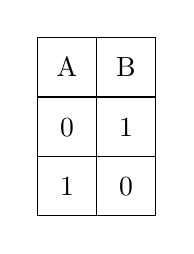
\begin{tikzpicture}
\matrix [
  matrix of nodes,
  row sep=-\pgflinewidth,
  column sep=-\pgflinewidth,
  nodes={draw, anchor=center, minimum size=.75cm},
  row 1/.style={row sep=0,nodes={}}
] {
  A & B \\
  0 & 1 \\
  1 & 0 \\
};
\end{tikzpicture}
\end{document}